\documentclass[10pt,twoside]{article}

\usepackage{amsmath,amssymb,amsthm}
\usepackage[subsection]{algorithm}
\usepackage{algpseudocode}
\renewcommand{\algorithmicrequire}{\textbf{Input:}\,}
\renewcommand{\algorithmicensure}{\textbf{Output:}}
\renewcommand{\algorithmicforall}{\textbf{for each}}
\newcommand{\Input}{\Require}
\newcommand{\Output}{\Ensure}
\newcommand{\ForEach}{\ForAll}
\usepackage{graphicx}
\usepackage{caption}

\newtheorem{definition}{Definition}[section]
\newtheorem{theorem}{Theorem}[section]
\numberwithin{equation}{section}

%
% Custom operator declarations
%
\DeclareMathOperator{\ZZ}{\mathbb{Z}}
\DeclareMathOperator{\CC}{\mathbb{C}}
\DeclareMathOperator{\KK}{\mathbb{C}}
\DeclareMathOperator{\PP}{\mathbb{P}}
\DeclareMathOperator{\hh}{\mathfrak{h}}
\DeclareMathOperator{\re}{\text{Re}}
\DeclareMathOperator{\im}{\text{Im}}

%
% Make marginpars smaller font
%
\let\oldmarginpar\marginpar
\renewcommand\marginpar[1]{\oldmarginpar[\scriptsize #1]{\scriptsize #1}}

\newcommand{\thchar}[2] {\begin{bmatrix}#1\\#2\end{bmatrix}}
\newcommand{\thcharsm}[2] {\left[ \begin{smallmatrix} #1 \\ #2 \end{smallmatrix} \right]}

\title{General Examination -- Algebro-Geometric
  Approach to Nonlinear Integrable Equations}

\author{
Chris Swierczewski\\
University of Washington\\
Department of Applied Mathematics}
\date{\today}

%%%%%%%%%%%%%%%%%%%%%%%%%%%%%%%%%%%%%%%%%%%%%%%%%%%%%%%%%%%%%%%%%%%%%%%%%%%%%%%
\begin{document}
%%%%%%%%%%%%%%%%%%%%%%%%%%%%%%%%%%%%%%%%%%%%%%%%%%%%%%%%%%%%%%%%%%%%%%%%%%%%%%%

\maketitle

%%%%%%%%%%%%%%%%%%%%%%%%%%%%%%%%%%%%%%%%%%%%%%%%%%%%%%%%%%%%%%%%%%%%%%%%%%%%%%%
\section{Introduction}
%%%%%%%%%%%%%%%%%%%%%%%%%%%%%%%%%%%%%%%%%%%%%%%%%%%%%%%%%%%%%%%%%%%%%%%%%%%%%%%

The Kadomtsev-Petviashvili (KP) equation is a partial differential
equation used to describe the surface height of a two-dimensional
periodic shallow water wave. Depending on certain physical
considerations [XXX], which we will ignore, one can derive either of the
following two equations
\begin{align}
  \left(-4u_t + 6uu_x + u_{xxx}\right)_x + 3\sigma^2 u_{yy} = 0, \quad
  \sigma^2 = -1, \label{eqn: KP1} \\
  \left(-4u_t + 6uu_x + u_{xxx}\right)_x + 3\sigma^2 u_{yy} = 0, \quad
  \sigma^2 = +1. \label{eqn: KP2}
\end{align}
where $u(x,y,t)$ is the surface height as a function of position $(x,y)$
and time $t$. In the sequel we will not rely on this distinction and
simply refer to the ``KP equation''.

%% \marginpar{
%%   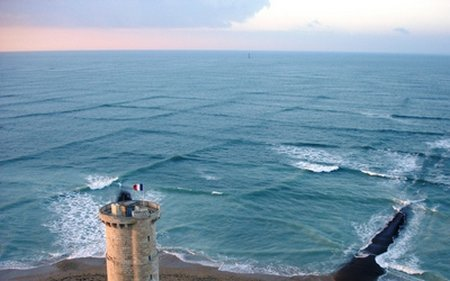
\includegraphics[width=\marginparwidth]{images/livekp.jpg}
%%   \captionof{figure}{KP waves off the coast of \^{I}le de R\'{e}, France.}
%% }

The KP equation admits a large family of quasiperiodic solutions of the
form
\begin{equation} \label{eqn: kpsol}
  u(x,y,t) = 2 \partial_x^2 \log \theta(Ux+Vy+Wt+z_0, \Omega)
\end{equation}
where $\theta$ is the Riemann theta function.

\begin{definition} \label{def: riemanntheta}
  The {\bf Riemann theta function} $\theta: \CC^g \times \hh_g \to \CC$
  is defined in terms of its Fourier series
  \begin{equation} \label{eqn: riemanntheta}
    \theta(z,\Omega) = \sum_{n \in \ZZ^g}
    e^{2 \pi i \left( \tfrac{1}{2} n \cdot \Omega n + n \cdot z \right)}.
  \end{equation}
  $\theta$ converges absolutely and uniformly on compact sets in $\CC
  \times \hh_g$ where $\hh_g$ is the space of all {\it ``Riemann
    matrices''} --- complex symmetric matrices with positive definite
  imaginary part.
\end{definition}

From the definition, we see that the Riemann theta function is periodic
in $z$ with integer periods and quasi-periodic in $z$ in the columns of
$\Omega$. In other words, if $m,n \in \ZZ^g$ then
\begin{equation} \label{eq: quasiperiodicity}
    \theta(z + m + \Omega n, \Omega) =
    e^{-2 \pi i \left( \tfrac{1}{2} n \cdot \Omega n + n \cdot z \right) }
    \theta(z, \Omega).
\end{equation}

A generalization of the Riemann theta function, involving a non-integer
shift in some of its arguments, is referred to as the Riemann theta
function with characteristics.

\begin{definition} \label{def: thetachar}
Let $\alpha,\beta \in [0,1)^{g}$. The {\bf Riemann theta function with
characteristic $\thcharsm{\alpha}{\beta}$} is defined as
\begin{align*}
  \theta\thchar{\alpha}{\beta}(z, \Omega) &=
  \sum_{n \in \mathbb{Z}^g}
  e^{2 \pi i \left( \tfrac{1}{2} (n+\alpha) \cdot \Omega (n+\alpha) +
    (n + \alpha) \cdot (z + \beta) \right) } \\
  &=
  e^{2\pi i \left( \tfrac{1}{2} \alpha \cdot \Omega \alpha +
    \alpha \cdot (z + \beta) \right)}
  \theta(z + \Omega \alpha + \beta, \Omega).
\end{align*}
\end{definition}

Note that $\theta \thcharsm{0}{0}(z,\Omega) = \theta(z,\Omega)$. See
\cite{DLMF,MumfordI07,MumfordII07} for further definitions and
properties of the Riemann theta function.

Returning to Equation \eqref{eqn: kpsol}, these solutions are the
so-called ``theta function solutions'' to the KP equation and families
of such solutions exist for every $g > 0$. In fact, the totality of
solutions of this form are dense the space of all periodic solutions to
KP. [XXX Marchenko and Ostrovskii?, see Dubrovin] The constants
$U,V,W,z_0 \in \CC^g$ and $\Omega \in \hh_g$ in \eqref{eqn: kpsol}, as
well as the ``genus'' $g$, are all determined from a Riemann surface
corresponding to a complex plane algebraic curve and any such curve can
produce a solution to KP. \cite{Dubrovin81} We will postpone precisely
how to determine these constants until more machinery is developed in
the following chapters.

\marginpar{Improve / elaborate upon the role of Abelian functions. This
  paragraph is a bit...I dunno.}

In general, periodic solutions to partial differential equations are
Abelian functions: doubly-periodic meromorphic functions defined on
Riemann surfaces [XXX]. Riemann theta functions play a central role in
the theory of Abelian functions in that all Abelian functions can be
written as a rational function of the Riemann theta function and its
derivatives. (Such as in the KP solution above.) Therefore, a primary
focus of study is the method of computation of these Abelian functions.

Riemann theta functions and algebraic curves are also used to solve
problems in optimization. In particular, the computation of bitangent
lines is useful for computations in optimization-related fields such as
algebraic geometry and convex optimization. In algebraic geometry,
bitangents can be used to represent smooth complex plane quartic curves
as both a symmetric determinant of a linear form (or, determinantal
representation) and a sum of three squares. \cite{PSV11} In convex
optimization, bitangents are used to construct a ``visibility complex''
which, in turn, is used to solve the shortest path problem in Euclidean
space \cite{PocchiolaVegter93}

\begin{definition} \label{def: bitangent}
  A {\bf bitangent} to a plane algebraic curve $C : f(x,y) = 0, f \in
  \CC[x,y]$ is a line $\mathcal{L} \subset \CC$ that lies tangent to $C$
  at at least two distinct points.
\end{definition}

By Bezout's Theorem, if a curve has a bitangent it necessarily must be
of degree at least four. \cite{Bezout1779} A result of Pl\"{u}cker
determines that a degree four complex curve admits exactly 28 complex
bitangents. \cite{Plucker34} In particular, Pl\"{u}cker showed that the
number of real bitangents of any quartic must be 28, 16, or fewer than
9. The connection between Riemann theta functions and the bitangent
lines of smooth quartics was known to Riemann \cite{Riemann76} and, in
fact, can be computed using the tools developed in this research. See
Figure \ref{fig: edge} for an example.

\marginpar{Note: this image will be replaced with the one generated by
  abelfunctions once I have it working properly again / once I find the
  image on my computer.}

\begin{figure}[t]
  \centering
  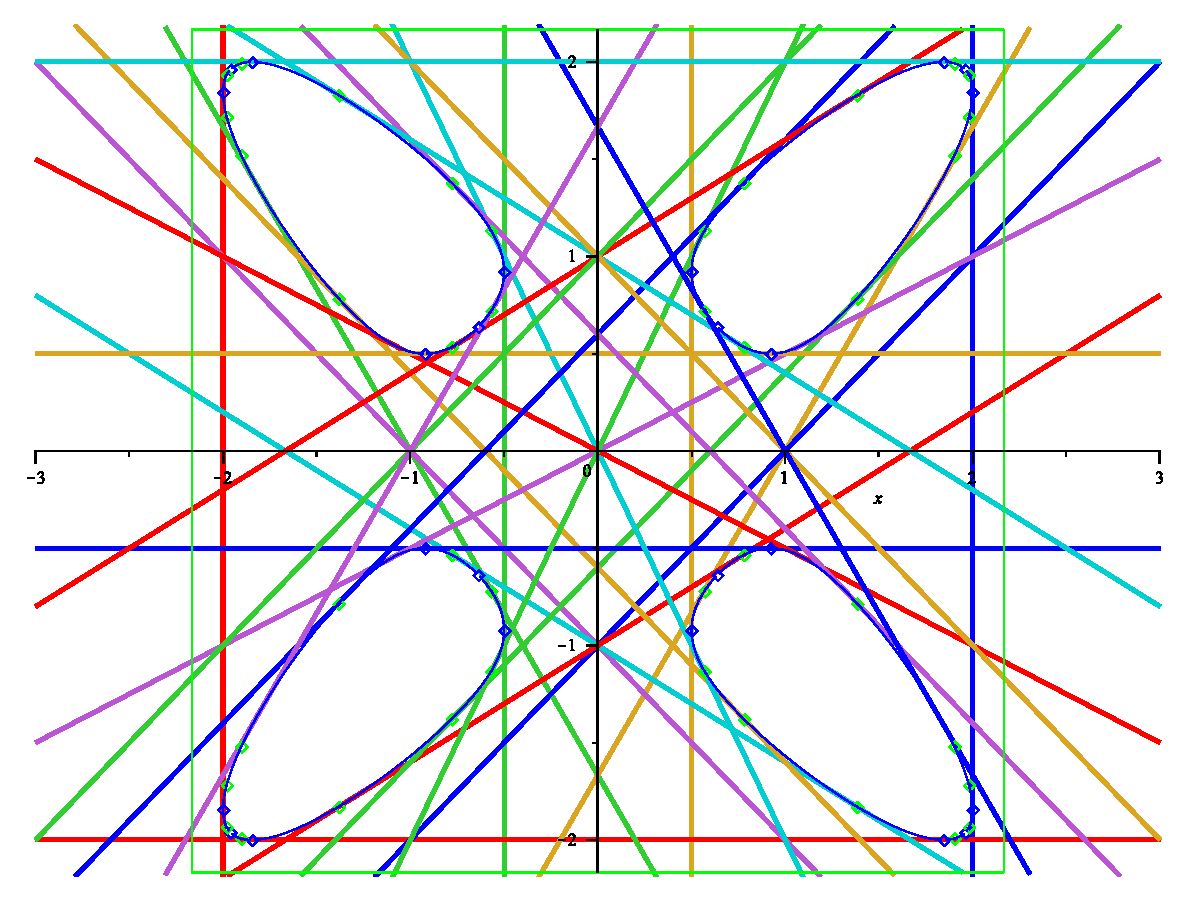
\includegraphics[width=0.8\textwidth]{images/edgequartic}
  \caption{The real graph of the Edge Quartic $C: f(x,y) = 25(x^4+y^4+1)
    - 34(x^2y^2+x^2+y^2) = 0$ and its 28 real bitangents. Note that four
    of them lie tangent $C$ at infinity. These lines were computed using
    the Riemann theta function.}
  \label{fig: edge}
\end{figure}

Finally, Riemann theta functions and algebraic curves can be used to
compute linear matrix representations of algebraic curves. A theorem
from classical algebraic geometry states that every homogenous
polynomial $f \in P^2\CC[x_0,x_1,x_2]$ can be written in the form
\[
   f(x_0,x_1,x_2) = \text{det}
   \left( A x_0 + B x_1 + C x_2 \right)
\]
where $A,B,C$ are symmetric complex matrices. These matrices can be
efficiently computed using Riemann theta functions. Furthermore, when
the polynomial has real coefficients then $A,B,C$ are symmetric real
matrices and such representations are important in the study of
spectrahedra --- the solution spaces of semidefinite
programs. \cite{PSV10}

The purpose of this research is to develop efficient and performant
algorithms for computing with Abelian functions on Riemann surfaces. The
computational tools developed in this research program have far-reaching
and varied applications.


%%%%%%%%%%%%%%%%%%%%%%%%%%%%%%%%%%%%%%%%%%%%%%%%%%%%%%%%%%%%%%%%%%%%%%%%%%%%%%%
\section{Complex Algebraic Geometry --- Period Matrices and the Abel Map}
%%%%%%%%%%%%%%%%%%%%%%%%%%%%%%%%%%%%%%%%%%%%%%%%%%%%%%%%%%%%%%%%%%%%%%%%%%%%%%%

In this section we give a brief introduction to the theory of complex
algebraic curves. We explain the concept of a period matrix and the Abel
map, a particular function from a Riemann surface to the complex
numbers.

%------------------------------------------------------------------------------
\subsection{Algebraic Curves and Riemann Surfaces}
%------------------------------------------------------------------------------

Primary references. \cite{Griffiths89}

A complex plane algebraic curve, $C$, is the zero locus of the
homogenization of a polynomial $f \in \CC[x,y]$. That is, given a
polynomial $f(x,y) = a_n(x) y^n + a_{n-1}(x)y^{n-1} + \cdots + a_0(x)$
its homogenization is the polynomial $F \in P^2\CC[x_0,x_1,x_2]$ where
\[
  f(x,y) = F(x,y,1)
  \quad \text{and} \quad
  F(x_0,x_1,x_2) = x_2^n f(x_0/x_2,x_1/x_2).
\]
($P^2\CC$ denotes two-dimensional complex projective space.) Therefore,
a complex plane algebraic curve is the set
\[
  C = \left\{
  (x_0,x_1,x_2) \in P^2\CC : F(x_0,x_1,x_2) = 0
  \right\}.
\]

There exists a close relationship between the study of compact Riemann
surfaces and that of algebraic curves. A Riemann surface $\tilde{C}$ is
simply a complex manifold of complex dimension one. This relationship is
embodied by the following two theorems.

\begin{theorem} \label{thm: normalization}
  {\it (Normalization Theorem.)} For any irreducible algebraic curve $C
  \subset P^2\CC$ there exists a compact Riemann surface $\tilde{C}$ and
  a holomorphic mapping
  \[
    \sigma : \tilde{C} \to P^2\CC
  \]
  such that $\sigma( \tilde{C} ) = C$ adn $\sigma$ is injective on the
  inverse image of the set of smooth points of $C$.
\end{theorem}

A Riemann surface together with the mapping $\sigma$ is called the {\it
  normalization of $C$}. Loosely speaking, the normalization theorem
states that an algebraic curve is a Riemann surface except at the
singular points.

%% In particular, any irreducible plane algebraic curves admits a
%% holomorphic parametric representation and the domain of definition of
%% this representation is a compact Riemann surface [[[]]]. The following
%% two theorems indeed show




%%%%%%%%%%%%%%%%%%%%%%%%%%%%%%%%%%%%%%%%%%%%%%%%%%%%%%%%%%%%%%%%%%%%%%%%%%%%%%%
\section{Computing Period Matrices of Algebraic Curves and the Abel Map}
%%%%%%%%%%%%%%%%%%%%%%%%%%%%%%%%%%%%%%%%%%%%%%%%%%%%%%%%%%%%%%%%%%%%%%%%%%%%%%%

In this section we will look at algorithmically computing period
matrices. Each subsection here examines in close detail a major
component of the algorithm and provides a theoretical overview of the
component, an algorithm for computing the component, and an example
presented in {\tt abelfunctions}, a Python software package


%------------------------------------------------------------------------------
\subsection{abelfunctions}
%------------------------------------------------------------------------------

%------------------------------------------------------------------------------
\subsection{Puiseux Series}
%------------------------------------------------------------------------------

%
\subsubsection*{Theory}
%

%
\subsubsection*{Algorithm}
%

\begin{algorithm}[h]
\caption{POLYGON --- Returns the Newton polygon of the polynomial $F =
  F(X,Y)$.}
\label{alg: puiseux-polygon}
\begin{algorithmic}[1]
\Input

$F,X,Y$ --- A polynomial.

$I$ --- If $I=0$, return the Newton polygon. If $I=1$, return only the
segments of the Newton polygon with negative slope. $I=1$ is used to
compute terms beyond the first of the Puiseux series.

\Output A set of lists $(q,m,l,\Phi)$ where
\begin{itemize}
  \item $q,m,l$ defines a line segment $\Delta: qj+mi=l$ in the $(i,j)$
    plane,
  \item $\Phi(Z) = \sum_{(i,j)\in\Delta} a_{ij} Z^{(i-i_0)/q} \in
    \CC[Z]$ where $i_0$ is the smallest value of $i$ such that there is
    a point $(i_0,j)\in\Delta$.
\end{itemize}

\Function{POLYGON}{$F,X,Y,I$}
  \State
\EndFunction
\end{algorithmic}
\end{algorithm}


\begin{algorithm}[h]
\caption{REGULAR --- Given the branching or singular part of a Puiseux
  series, computes the regular part of the series.}
\label{alg: puiseux-regular}
\begin{algorithmic}[1]
\Input

$S$ --- a finite set of pairs $\{(\pi_k,F_k)\}$

$X,Y$ --- the dependent and independent variables, respectively

$H$ --- bound on the number of desired terms of the series

\Output $R$ --- a finite set of pairs $\{(\pi_k,F_k)\}$ containing at
least $H$ terms

\Function{Regular}{$S,X,Y,H$}
  \State $R \leftarrow ()$
  \ForEach{$(\pi,F)$ {\bf in} $S$}
    \While{$\text{len}(\pi) < H$}

      \State $m \leftarrow \text{min} \{ j \; /$
      \Call{COEFFICIENT}{$F,0,j$} $ \; | \; j \neq 0 \}$

      \State $\beta \leftarrow$ \Call{COEFFICIENT}{$F,0,m$} /
      \Call{COEFFICIENT}{$F,1,0$}

      \State $\tau \leftarrow (1,1,m,\beta)$
      \State $\pi \leftarrow \pi \cup \{\tau\}$
      \State $F \leftarrow$ \Call{NEWPOLYNOMIAL}{$F,\tau,m$}
    \EndWhile
    \State $R \leftarrow R \cup \{\pi\}$
  \EndFor
\EndFunction
\end{algorithmic}
\end{algorithm}


\subsubsection*{Examples}
%

%------------------------------------------------------------------------------
\subsection{Singularities}
%------------------------------------------------------------------------------

%
\subsubsection*{Theory}
%
%
\subsubsection*{Algorithm}
%
%
\subsubsection*{Examples}
%

%------------------------------------------------------------------------------
\subsection{Holomorphic Differentials}
%------------------------------------------------------------------------------

%
\subsubsection*{Theory}
%



%
\subsubsection*{Algorithm}
%
%
\subsubsection*{Examples}
%

%------------------------------------------------------------------------------
\subsection{Analytic Continuation}
%------------------------------------------------------------------------------

%
\subsubsection*{Theory}
%

A path on a Riemann surface is a continuous map $\gamma : [0,1] \to C
\subset \CC^2$. That is, if $\gamma(t) = (x_\gamma(t), y_\gamma(t))$
then $f(x(t),y(t)) = 0$ for all $t \in [0,1]$.


%
\subsubsection*{Algorithm}
%

Since analytic continuation is repeatedly performed when computing
period matrices it is important to make it performant.

Often, a path in $\CC_x$, $x_\gamma$, will be specified, such as via the
{\sc monodromy() or homology()} functions, and the corresponding
$y$-values lying above need to be determined. A naive approach to doing
so is to use a numerical root finder.

An alternate approach, which is the one used here, is to use Newton's
method --- given $x_\gamma(t_k)$ and some $y_{\gamma,j}(t_k)$ lying
above determine $y_{\gamma,j}(t_{k+1})$ above $x_\gamma(t_{k+1})$.

%
\subsubsection*{Examples}
%

%------------------------------------------------------------------------------
\subsection{Monodromy}
%------------------------------------------------------------------------------

%
\subsubsection*{Theory}
%
%
\subsubsection*{Algorithm}
%
%
\subsubsection*{Examples}
%

%------------------------------------------------------------------------------
\subsection{Homology}
%------------------------------------------------------------------------------

%
\subsubsection*{Theory}
%
%
\subsubsection*{Algorithm}
%
%
\subsubsection*{Examples}
%

%------------------------------------------------------------------------------
\subsection{Period Matrices}
%------------------------------------------------------------------------------

%
\subsubsection*{Theory}
%
%
\subsubsection*{Algorithm}
%
%
\subsubsection*{Examples}
%

%------------------------------------------------------------------------------
\subsection{The Abel Map}
%------------------------------------------------------------------------------

%
\subsubsection*{Theory}
%
%
\subsubsection*{Algorithm}
%
%
\subsubsection*{Examples}
%

%%%%%%%%%%%%%%%%%%%%%%%%%%%%%%%%%%%%%%%%%%%%%%%%%%%%%%%%%%%%%%%%%%%%%%%%%%%%%%%
\section{Periodic Solutions to Nonlinear Integrable Equations}
%%%%%%%%%%%%%%%%%%%%%%%%%%%%%%%%%%%%%%%%%%%%%%%%%%%%%%%%%%%%%%%%%%%%%%%%%%%%%%%

%------------------------------------------------------------------------------
\subsection{Example: The Kadomtsev--Petviashvili Equation}
%------------------------------------------------------------------------------

%------------------------------------------------------------------------------
\subsection{Geometry of Integrable Equations}
%------------------------------------------------------------------------------


%%%%%%%%%%%%%%%%%%%%%%%%%%%%%%%%%%%%%%%%%%%%%%%%%%%%%%%%%%%%%%%%%%%%%%%%%%%%%%%
\section{Future Work}
%%%%%%%%%%%%%%%%%%%%%%%%%%%%%%%%%%%%%%%%%%%%%%%%%%%%%%%%%%%%%%%%%%%%%%%%%%%%%%%

%------------------------------------------------------------------------------
\subsection{Periodic Solutions of Integrable Equations}
%------------------------------------------------------------------------------

%------------------------------------------------------------------------------
\subsection{Fay's Prime Form}
%------------------------------------------------------------------------------

%------------------------------------------------------------------------------
\subsection{The Constructive Schottky Problem}
%------------------------------------------------------------------------------


%%%%%%%%%%%%%%%%%%%%%%%%%%%%%%%%%%%%%%%%%%%%%%%%%%%%%%%%%%%%%%%%%%%%%%%%%%%%%%%
\section{Bibliography}
%%%%%%%%%%%%%%%%%%%%%%%%%%%%%%%%%%%%%%%%%%%%%%%%%%%%%%%%%%%%%%%%%%%%%%%%%%%%%%%


\bibliographystyle{amsalpha}
\bibliography{general-exam}


%%%%%%%%%%%%%%%%%%%%%%%%%%%%%%%%%%%%%%%%%%%%%%%%%%%%%%%%%%%%%%%%%%%%%%%%%%%%%%%
\end{document}
%%%%%%%%%%%%%%%%%%%%%%%%%%%%%%%%%%%%%%%%%%%%%%%%%%%%%%%%%%%%%%%%%%%%%%%%%%%%%%%
